\documentclass[a4paper,10pt]{esannV2}
\usepackage[T1]{fontenc}
\usepackage[utf8]{inputenc}
\usepackage{graphicx,amsmath,amssymb,array}
\setlength{\oddsidemargin}{18.6mm}\setlength{\evensidemargin}{18.6mm}
\setlength{\topmargin}{26.6mm}\setlength{\headheight}{0pt}\setlength{\headsep}{0pt}
\setlength{\textwidth}{122mm}\setlength{\textheight}{193mm}
\hoffset=0pt\voffset=0pt
\newcommand{\GloveGain}{18.8}
\newcommand{\CocoGain}{15.2}

\newcommand{\E}{\mathbb{E}}\newcommand{\Prb}{\mathbb{P}}
\begin{document}
\title{Forecasting Recall Feasibility Before Calibration:\\A Held-Out Diagnostic Study of Capped IVF Retrieval}
\author{Kavyasree Nunna\vspace{.3cm}\\Affiliation and postal address to be confirmed before submission}
\maketitle
\begin{abstract}
Hard retrieval budgets and limited calibration evidence create different obstacles
to recall certification. We test whether centroid geometry helps distinguish
these obstacles before collecting calibration labels. Matched tree
models predict maximal-prefix recall losses using design labels and either
occupancy features or additional geometry. Frozen five-seed pilots trigger
confirmation on separate queries from GloVe and COCO CLIP retrieval. Geometry
reduces severity prediction error, but does not confer a distribution-free safety
guarantee. Operational gains vary across workloads; source-level lookahead costs
also vary across seeds. We release protocols, disjoint query roles, negative
findings, and exact traces while retaining limits on novelty and generalization.
\end{abstract}
\section{A diagnostic question, not a new calibration theorem}
Recall calibration is useful only when a search policy can satisfy the requested
risk at the permitted work budget. ConANN already provides adaptive IVF recall
calibration~\cite{conann}, and LTT/Pareto Testing already address risk-constrained
configuration selection~\cite{ltt,pareto}. Feasibility diagnostics also have prior
work outside retrieval~\cite{feasibility}. Merely applying these tools to another
loss is not our claimed contribution.

We investigate a narrower empirical question: \emph{does design-trained query
geometry improve predictions of the best recall attainable by a fixed capped
prefix class, beyond cap and occupancy information alone?} Such predictions
could support triage before expensive additional labeling, but remain fallible
forecasts. We separately examine actual risk certification and executed-work
accounting; prediction accuracy cannot substitute for either.

The study extends earlier unsuccessful adaptive-calibration experiments.
We freeze the protocol, add cross-modal retrieval and evaluate fresh queries.
It confirms one prespecified diagnostic criterion, retains a failed accounting
gate, and makes no claim of a new statistical algorithm or optimal search policy.

\newpage
\section{Retrieval floors, evidence, and forecast targets}
Fix $N=10{,}000$ corpus vectors, an IVF index with $M=64$ lists ordered by centroid
distance, and $k=10$. Lists are scanned completely. For exact neighbors $T_k(q)$
and candidate union $A_p(q)$, define
\begin{equation}
 L(q,p)=1-\frac{|T_k(q)\cap A_p(q)|}{k},\qquad
 C(q,p)=64+\sum_{i=1}^{p}|I_i(q)|.
\end{equation}
The cap is $B=64+\lfloor bN\rfloor$, with
$b\in\{.05,.10,.25,.50,1\}$. Empty prefixes have loss $1$. Every admissible
whole-list prefix policy obeys $\pi(q)\le p_B(q)$, where
\begin{equation}
 p_B(q)=\max\{p:C(q,p)\le B\},\qquad L_B(q)=L(q,p_B(q)).
\end{equation}
Nested candidates imply $L(q,\pi(q))\ge L_B(q)$ pointwise, including for
nondecreasing severity transforms and conditional averages. This elementary
floor is class-specific; it is not a knapsack hardness theorem or an impossibility
result for graphs, partial lists or alternative probe orders.

Each diagnostic predicts the three bounded targets
\begin{equation}
 Z_B(q)=\big(L_B(q),\ \mathbf{1}\{L_B(q)>.20\},\
 \mathbf{1}\{L_B(q)>.50\}\big).
\end{equation}
Four fixed overlapping groups comprise all queries and the upper 20\%, 10\%
and 5\% of design-defined centroid ambiguity. A workload/group regime is
empirically feasible if its three average targets are at most $(.10,.10,.05)$.
We call a diagnostic prediction an \emph{admission} only when all three predicted
averages meet these thresholds. It is not a certificate.

Certification uses standard fixed-sequence LTT: the maximum of 12 one-sided
Chernoff p-values at $.025$. For constraint $j$ with target $a_j$, group count
$n_j$ and bounded empirical risk $\widehat R_j$, the test is
\begin{equation}
p_j=\begin{cases}
\exp\{-n_j\operatorname{kl}(\widehat R_j\Vert a_j)\},&\widehat R_j<a_j,\ n_j>0,\\
1,&\text{otherwise}.
\end{cases}
\end{equation}
Here $\operatorname{kl}$ is binary relative entropy. Confidence is per fixed
method/cap, not simultaneous over the displayed grid. Prospective safety requires
a design-fixed path and a matching within-group query law; these source-law
assumptions are not replaced by a predictor's accuracy.
A reverse floor test at $.025/12$ can supply an
infeasibility witness; otherwise inability to certify is \emph{unknown}.
Zero events for a $.05$ severity target require at least
$\lceil\log(.025)/\log(.95)\rceil=72$ group examples under this test.
This is a count requirement of the implemented procedure, not a universal
lower bound or an explanation for every unknown. More evidence can reveal
infeasibility instead of producing a certificate.

\newpage
\section{Frozen pilots and confirmation protocol}
We use normalized GloVe-25 embeddings~\cite{glove} and author-released COCO
text-to-image CLIP ViT-B/16 vectors~\cite{clip,cocodata}. The latter has 512
dimensions, image corpus vectors and caption queries. Each workload uses five
corpus/index seeds, $0$--$4$. All runs share fixed query-role assignments:
500 design, 2,000 calibration, 500 pilot and 2,000 confirmation queries.
The 24,771 GloVe training queries inspected in previous calibration studies
were excluded before assigning new roles; previous official final TEST queries
were never loaded. Recall concerns exact embedding neighbors, not semantic
relevance judgments or downstream answer quality.

Both diagnostics are standard ExtraTrees regressors~\cite{trees} with 64 trees.
The occupancy control uses cap fraction, feasible prefix fraction, used corpus
fraction and next-list fraction. Geometry adds centroid ambiguity, scaled nearest
centroid distance, distance spread and two list-radius ratios. These features
use no query's exact neighbors at prediction time; training still uses design
labels. Both models receive the same four depth/leaf settings, selected on
300/200 design queries before refitting on all 500. Query identities are separated
before expansion across caps.

H1 requires at least 10\% severity Brier-error reduction over occupancy in
at least 4/5 seeds on both datasets, nonzero admissions and at most 10\% empirical
false admissions among admitted regimes in each passing seed. The Brier score
averages squared errors for the two severity indicators over queries and caps.
Pilots passed in 5/5 GloVe and 4/5 COCO seeds. Source, protocol, pilot outputs
and selected settings were then hashed before confirmation outcomes.

An input-only audit found repeated COCO vectors under different row IDs.
Before confirmation labeling, six repeated vectors were replaced using a fixed
unused-row order. Confirmation vectors are unique and disjoint in value from
design, calibration and pilot roles. The small pilot overlap is disclosed, with
a duplicate-excluded score sensitivity; no model was retuned.

\begin{table}[!h]
\centering\small\setlength{\tabcolsep}{3pt}
\begin{tabular}{lrrrr}
\hline
Data & Occupancy & Geometry & Gain (\%) & Gate \\
\hline
GloVe & $0.0578\pm0.0024$ & $0.0469\pm0.0014$ & $18.8\pm1.9$ & 5/5 \\
COCO CLIP & $0.0949\pm0.0034$ & $0.0804\pm0.0029$ & $15.2\pm2.6$ & 4/5 \\
\hline
\end{tabular}

\caption{Fresh confirmation: Brier error and relative gain, mean $\pm$ seed SD.
Gate counts repeat the unchanged full H1 criterion. Five seeds share query pools;
they are not independent external datasets.}
\end{table}

Separately, post-confirmation controls used only the old pilot, without retuning.
Shuffling geometry raised mean Brier error from .0504 to .0618 on GloVe and
from .0823 to .0964 on COCO. This supports predictive information beyond merely
adding feature dimensions, but mechanistic attribution remains exploratory.

\newpage
\section{Decision consequences and certification boundaries}
Geometry improves mean prediction error by \GloveGain\% on GloVe and
\CocoGain\% on COCO. The confirmation criterion passes in 5/5 and 4/5 seeds.
COCO seed 0 improves Brier error by 12.2\% yet fails because one of nine admissions
is false ($11.1\%$). We retain this failure rather than relax the threshold.

\begin{table}[!h]
\centering\small\setlength{\tabcolsep}{3pt}
\begin{tabular}{llrrrr}
\hline
Data & Diagnostic & Admit & False admit & False refuse & Correct \\
\hline
GloVe & Occupancy & 60 & 0 & 0 & 100 \\
GloVe & Geometry & 60 & 0 & 0 & 100 \\
COCO CLIP & Occupancy & 52 & 10 & 0 & 90 \\
COCO CLIP & Geometry & 43 & 1 & 0 & 99 \\
\hline
\end{tabular}

\caption{Confirmation decisions over five caps, four groups and five index seeds:
100 \emph{dependent} regimes per dataset. False admission means predicted feasible
but empirically infeasible. False refusal is the converse. No binomial-trial or
population error-bound interpretation is justified by these totals.}
\end{table}

On GloVe, lower prediction error does not change decisions: the simpler control
already classifies all evaluated regimes correctly. On COCO, geometry avoids
nine false admissions without increasing false refusals in this workload.
This is an observed engineering distinction, not a guaranteed reduction in
deployment failures or labeling cost.

\begin{figure}[!h]
\centering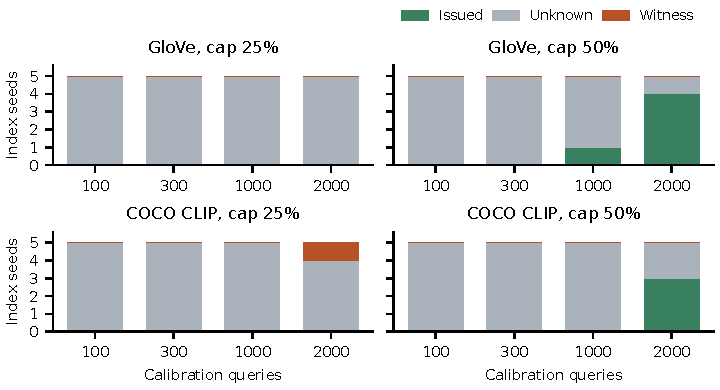
\includegraphics[width=\linewidth]{generated/figure_certification.pdf}
\caption{Uniform-LTT status by calibration count and cap, all five index seeds.
Unknown is distinct from a calibrated infeasibility witness. More labels can
support a witness, not just issuance. The same labels are shared across methods
and caps; labeling costs cannot be multiplied by the number of displayed cases.}
\end{figure}

\newpage
\section{Robustness, accounting audit and scope of evidence}
\begin{figure}[!h]
\centering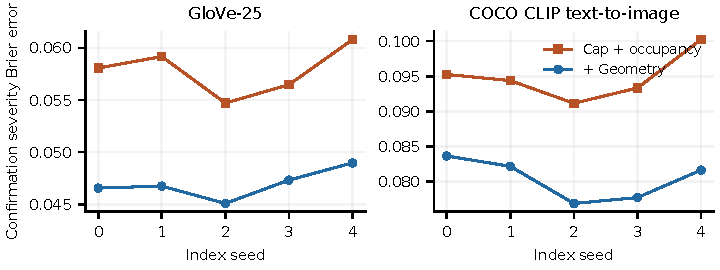
\includegraphics[width=\linewidth]{generated/figure_forecasts.pdf}
\caption{Fresh-query Brier error for each index realization. Both diagnostics use
identical design labels and tuning budgets. A better forecast is not necessarily
a better admission decision, as GloVe demonstrates.}
\end{figure}

All ten index runs were retained in both phases. Each phase has 600 cases
spanning caps, calibration counts and methods, plus 2,400 group rows. Checks rebuilt
group assignments and verified raw/summary agreement, hard caps, score averages
and returned/executed work. Paired query bootstraps use 2,000 resamples, keeping
each query's caps together. They quantify conditional variation on these shared
datasets, not independent-study uncertainty or universal safety.

Uniform, design-cell-shift and author-score paths are additionally calibrated
under identical LTT group/tail constraints, with calibration counts 100, 300, 1000
and 2000. At the primary 25\% cap no such path issued; an unissued diagnostic output
is never reported as a certified deployed policy. The forecast comparison
therefore does not claim to improve certified retrieval latency.

H2 separately tested executed versus returned-prefix work. In the pinned ConANN
source, an extra list may be scanned before the previous result is restored.
We compiled the exact scalar stop expressions and passed 10,000 differential
checks plus live synthetic retrieval controls. The prespecified material-overhead
pilot gate passed only 3/5 GloVe seeds versus 5/5 COCO seeds, hence failed across
workloads. We do not rescue that hypothesis using confirmation statistics.

Crucially, the author's native distance counter already counts executed scans;
this is \emph{not} evidence that published ConANN latency is wrong. Our portable
score adapter uses discrete CRC selection rather than GSL root solving, a fixed
normalized-distance scale and locally implemented IVF. Isolated numerical
dependencies resolved configuration, but the unmodified full engine fails on
this Windows/MinGW toolchain at a POSIX allocation call. No full author-code
performance reproduction is claimed.

\newpage
\section{Conclusions and remaining publication limits}
The confirmed result is scoped: adding geometry to a matched design-trained
occupancy predictor improves severity-risk forecasts on two retrieval workloads.
It changes admission decisions on COCO, while GloVe shows that score improvements
alone need not change an operational choice. Retrieval feasibility, statistical
evidence and executed compute must remain separate quantities.

This is an empirical diagnostic contribution candidate, not a new conformal
algorithm, formal admission guarantee or original impossibility theorem. The
same two public query sources are reused across index seeds. Corpus size is
10,000, models are fixed, and semantic/OOD shift is untested. The rarest groups
still have limited observations. Larger corpora, additional encoders, full
ConANN/Faiss validation and a measured end-to-end diagnostic deployment remain
necessary for broader claims. A large recorded wall-clock outlier is retained;
timings on the loaded host do not establish hardware deadlines. No acceptance
or exhaustive novelty claim is made.

Frozen code, role IDs, hashes, all outcomes, bootstrap intervals and attempt
ledgers accompany this draft. Earlier failures are retained separately. Fresh
confirmation was opened only after the pilot gate; prior official reserved TEST
queries and thousands of unused COCO queries remain unexamined.

\begin{thebibliography}{8}
\raggedright
\bibitem{conann} S. Horchidan et al. ConANN: Conformal Approximate Nearest
Neighbor Search. \emph{PVLDB},19(1):29--42,2025.
\bibitem{ltt} A. N. Angelopoulos et al. Learn then Test: Calibrating Predictive
Algorithms to Achieve Risk Control. arXiv:2110.01052,2021.
\bibitem{pareto} B. Laufer-Goldshtein et al. Efficiently Controlling Multiple
Risks with Pareto Testing. \emph{ICLR},2023.
\bibitem{feasibility} V. Kotte. When Can Conformal Risk Control Certify LLM
Outputs? Bounds, Impossibility, and Adaptation for Structured Generation.
arXiv:2606.29054,2026. Preprint.
\bibitem{glove} J. Pennington, R. Socher and C. D. Manning. GloVe: Global
Vectors for Word Representation. \emph{EMNLP},1532--1543,2014.
\bibitem{clip} A. Radford et al. Learning Transferable Visual Models From
Natural Language Supervision. \emph{ICML},8748--8763,2021.
\bibitem{cocodata} F. Carrara. COCO CLIP features, \texttt{str-encoders}
release v0.1.3. GitHub dataset artifact; accessed 30 October 2026.
\bibitem{trees} P. Geurts, D. Ernst and L. Wehenkel. Extremely randomized
trees. \emph{Machine Learning},63:3--42,2006.
\end{thebibliography}
\end{document}
